\documentclass[a4paper]{report}
\setlength{\headheight}{12.0pt}
\usepackage[T2A]{fontenc}
\usepackage[utf8]{inputenc}
\usepackage[russian,english]{babel}
\usepackage[left=25mm, top=20mm, right=25mm, bottom=30mm, nohead, nofoot]{geometry}
\usepackage{amsmath,amsfonts,amssymb} % математический пакет
\usepackage{fancybox,fancyhdr}
\usepackage{xcolor}
\usepackage{hyperref}
\usepackage{tkz-euclide}
\usepackage{enumitem}
\usepackage{amsmath}
\usepackage{pgfplots}
\usepackage{float}
\usepackage{fvextra}
\usepackage[cache=false]{minted}
\usepackage[figurename=Изображение]{caption}
\captionsetup[table]{name=Таблица}
\usemintedstyle{vs}

\hypersetup{colorlinks=true, allcolors=[RGB]{010 090 200}} % цвет ссылок
\newcommand{\lr}[1]{\left({#1}\right)} % команда для скобок
\pagestyle{fancy}
\fancyhf{}
\renewcommand{\headrulewidth}{0pt}
\fancyfoot[R]{\thepage}
\fancypagestyle{plain}{
    \fancyhf{}
    \fancyfoot[R]{\thepage}
    \renewcommand{\headrulewidth}{0pt}
}
\setcounter{page}{1} % счетчик нумерации страниц
\headsep=10mm
\definecolor{green_india}{HTML}{138808} % INDIA GREEN
\definecolor{green_light}{HTML}{90EE90} % LIGHT GREEN
\definecolor{green_slimy}{HTML}{299617} % SLIMY GREEN
\makeatletter
\def\@seccntformat#1{\csname #1ignore\expandafter\endcsname\csname the#1\endcsname\quad}
\let\latex@numberline\numberline
\def\numberline#1{\if\relax#1\relax\else\latex@numberline{#1}\fi}
\makeatother
\renewcommand{\thesection}{\arabic{section}.}
\renewcommand{\thesubsection}{\arabic{section}.\arabic{subsection}}

\begin{document}
\section{Диаграмма классов}
\begin{figure}[H]
    \centering
    \includegraphics[width=\textwidth]{Диаграмма классов.png}
\end{figure}
\begin{enumerate}
    \item \textbf{Product (Продукт)} - предназначен, для представления товара, который доступен для покупки;
    \item \textbf{Order (Заказ)} - класс, который хранит всю нужную информацию для заказа;
    \item \textbf{Review (Отзыв)} - отзыв заказа;
    \item \textbf{\textit{User (Пользователь)}} - абстрактный класс, который хранит в себе общую информацию;
    \item \textbf{Client (Клиент)} - класс, который осуществляет действия клиента;
    \item \textbf{\textit{Employ (Сотрудник)}} - абстрактный класс, который хранит в себе общую информацию сотрудника;
    \item \textbf{Manager (Менеджер)} - класс, который осуществляет работу менеджера;
    \item \textbf{Courier (Курьер)} - класс, который осуществляет работу курьера;
\end{enumerate}
\newpage
\section{Диаграмма последовательностей}
\subsection{CreateOrder}
\begin{figure}[H]
    \centering
    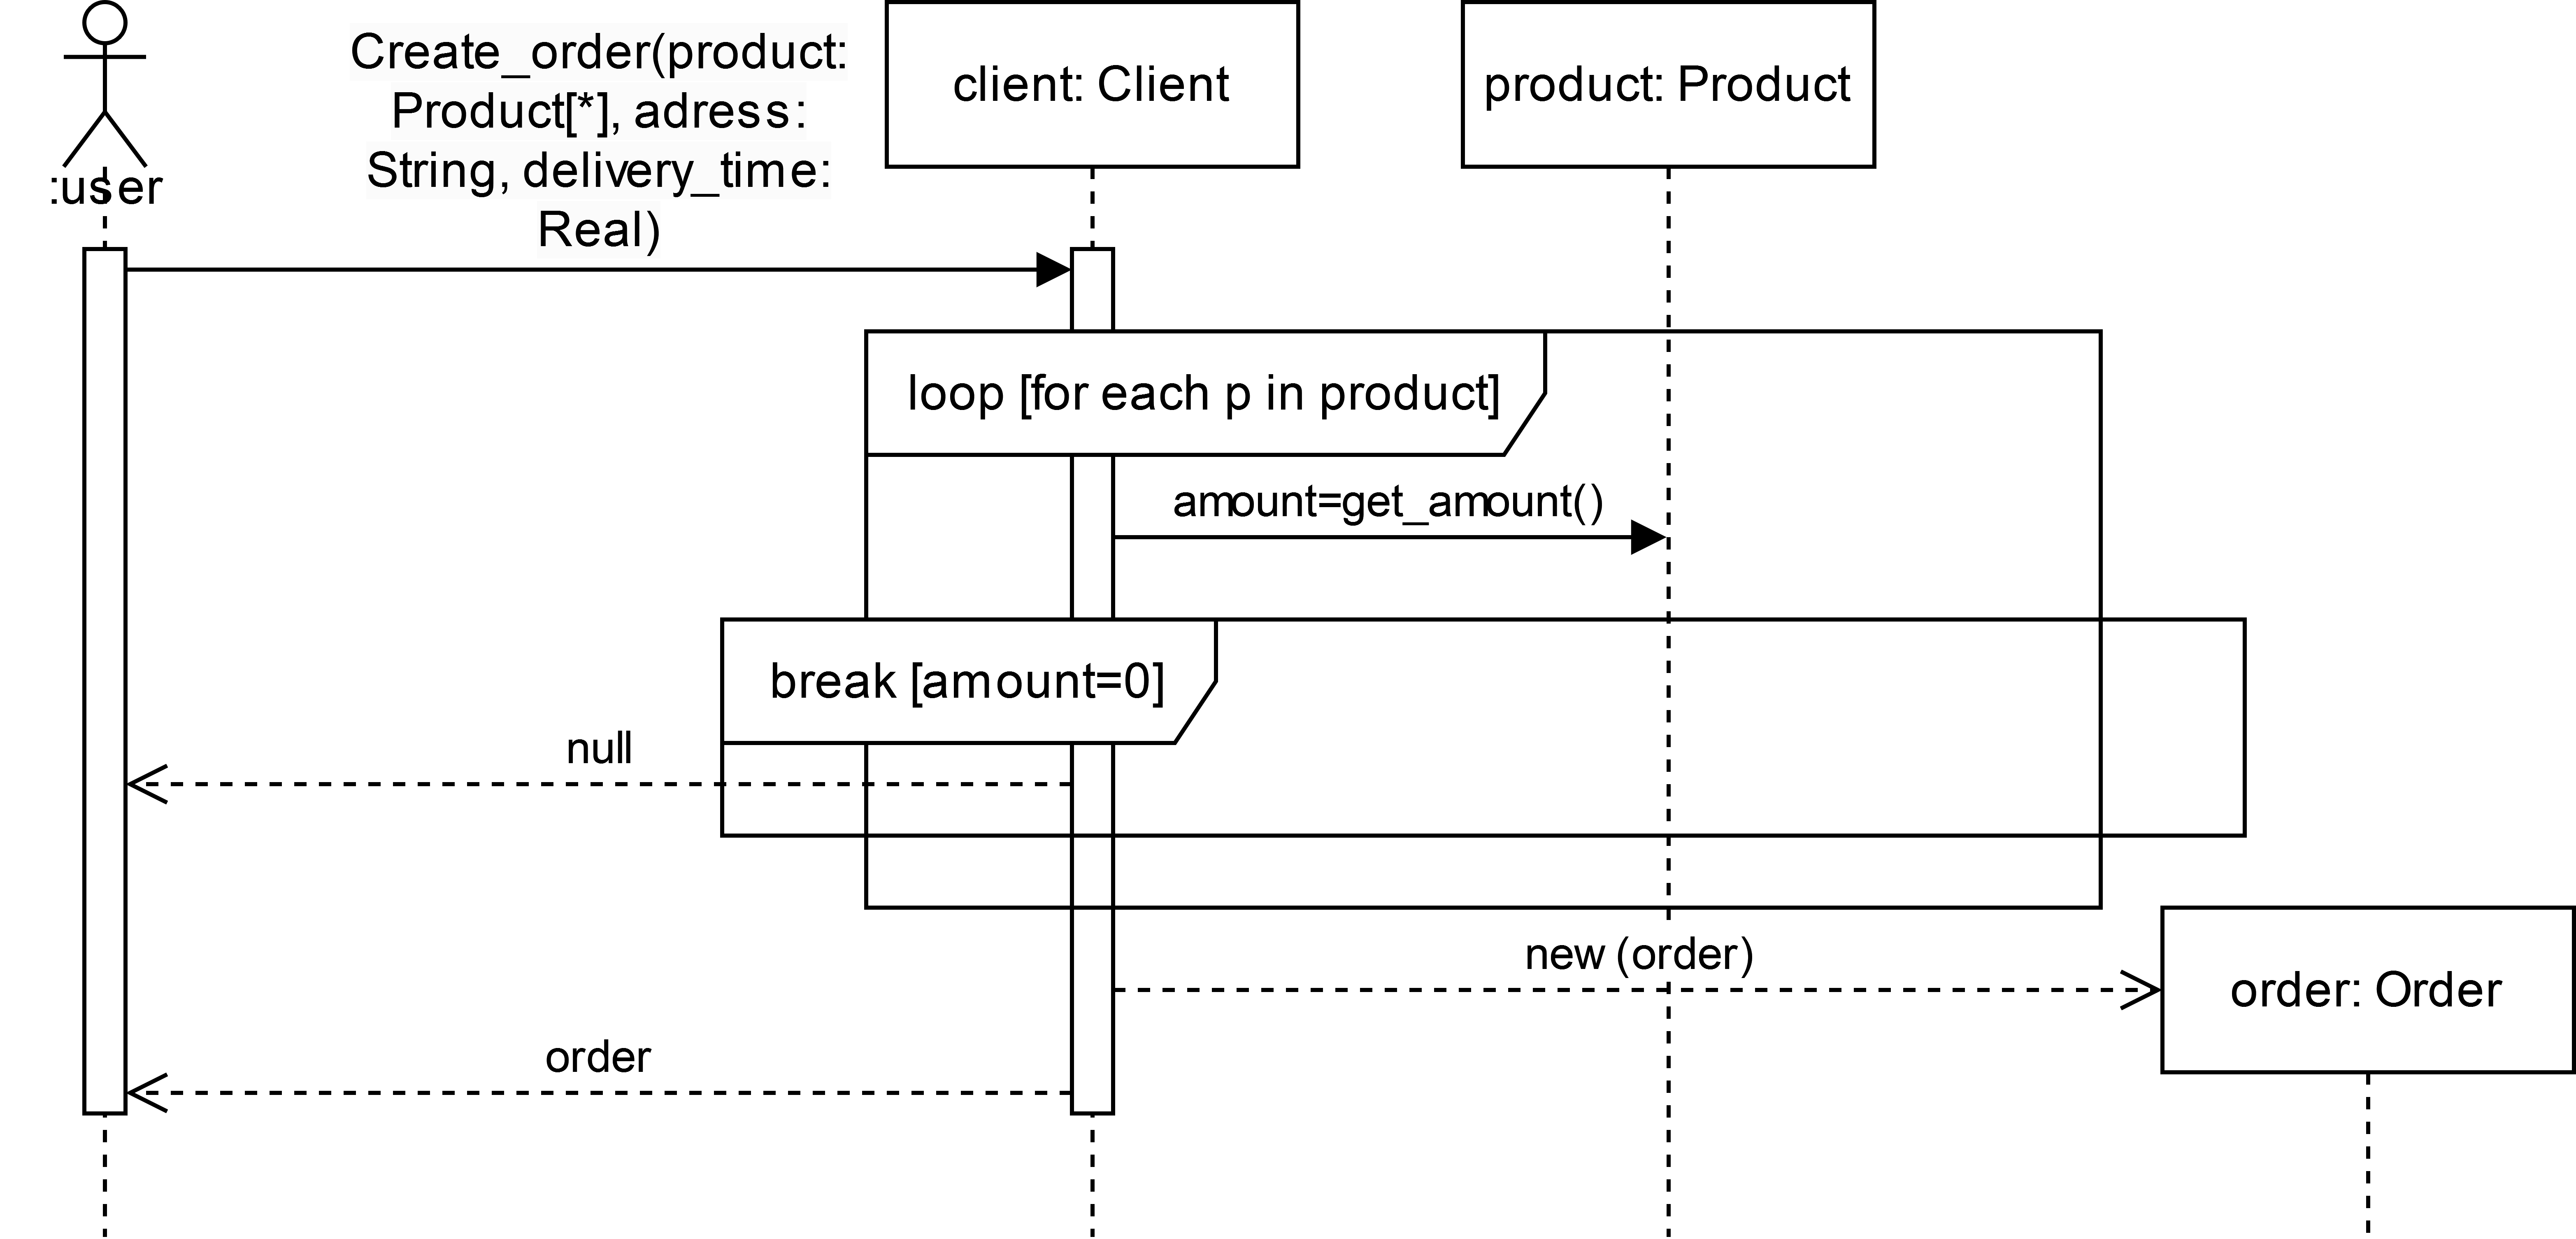
\includegraphics[width=\textwidth]{Диаграмма последовательностей create_order.png}
\end{figure}
User вызывает метод CreateOrder у объекта client класса Client. Посредством цикла проверяется наличие продукта с помощью использования метода get\_amount. Если продукта нет в наличие то заказ не создаётся и происходит выход из цикла посредством break. Если все продукты есть в наличие то будет создан заказ Order

\subsection{CreateReview}
\begin{figure}[H]
    \centering
    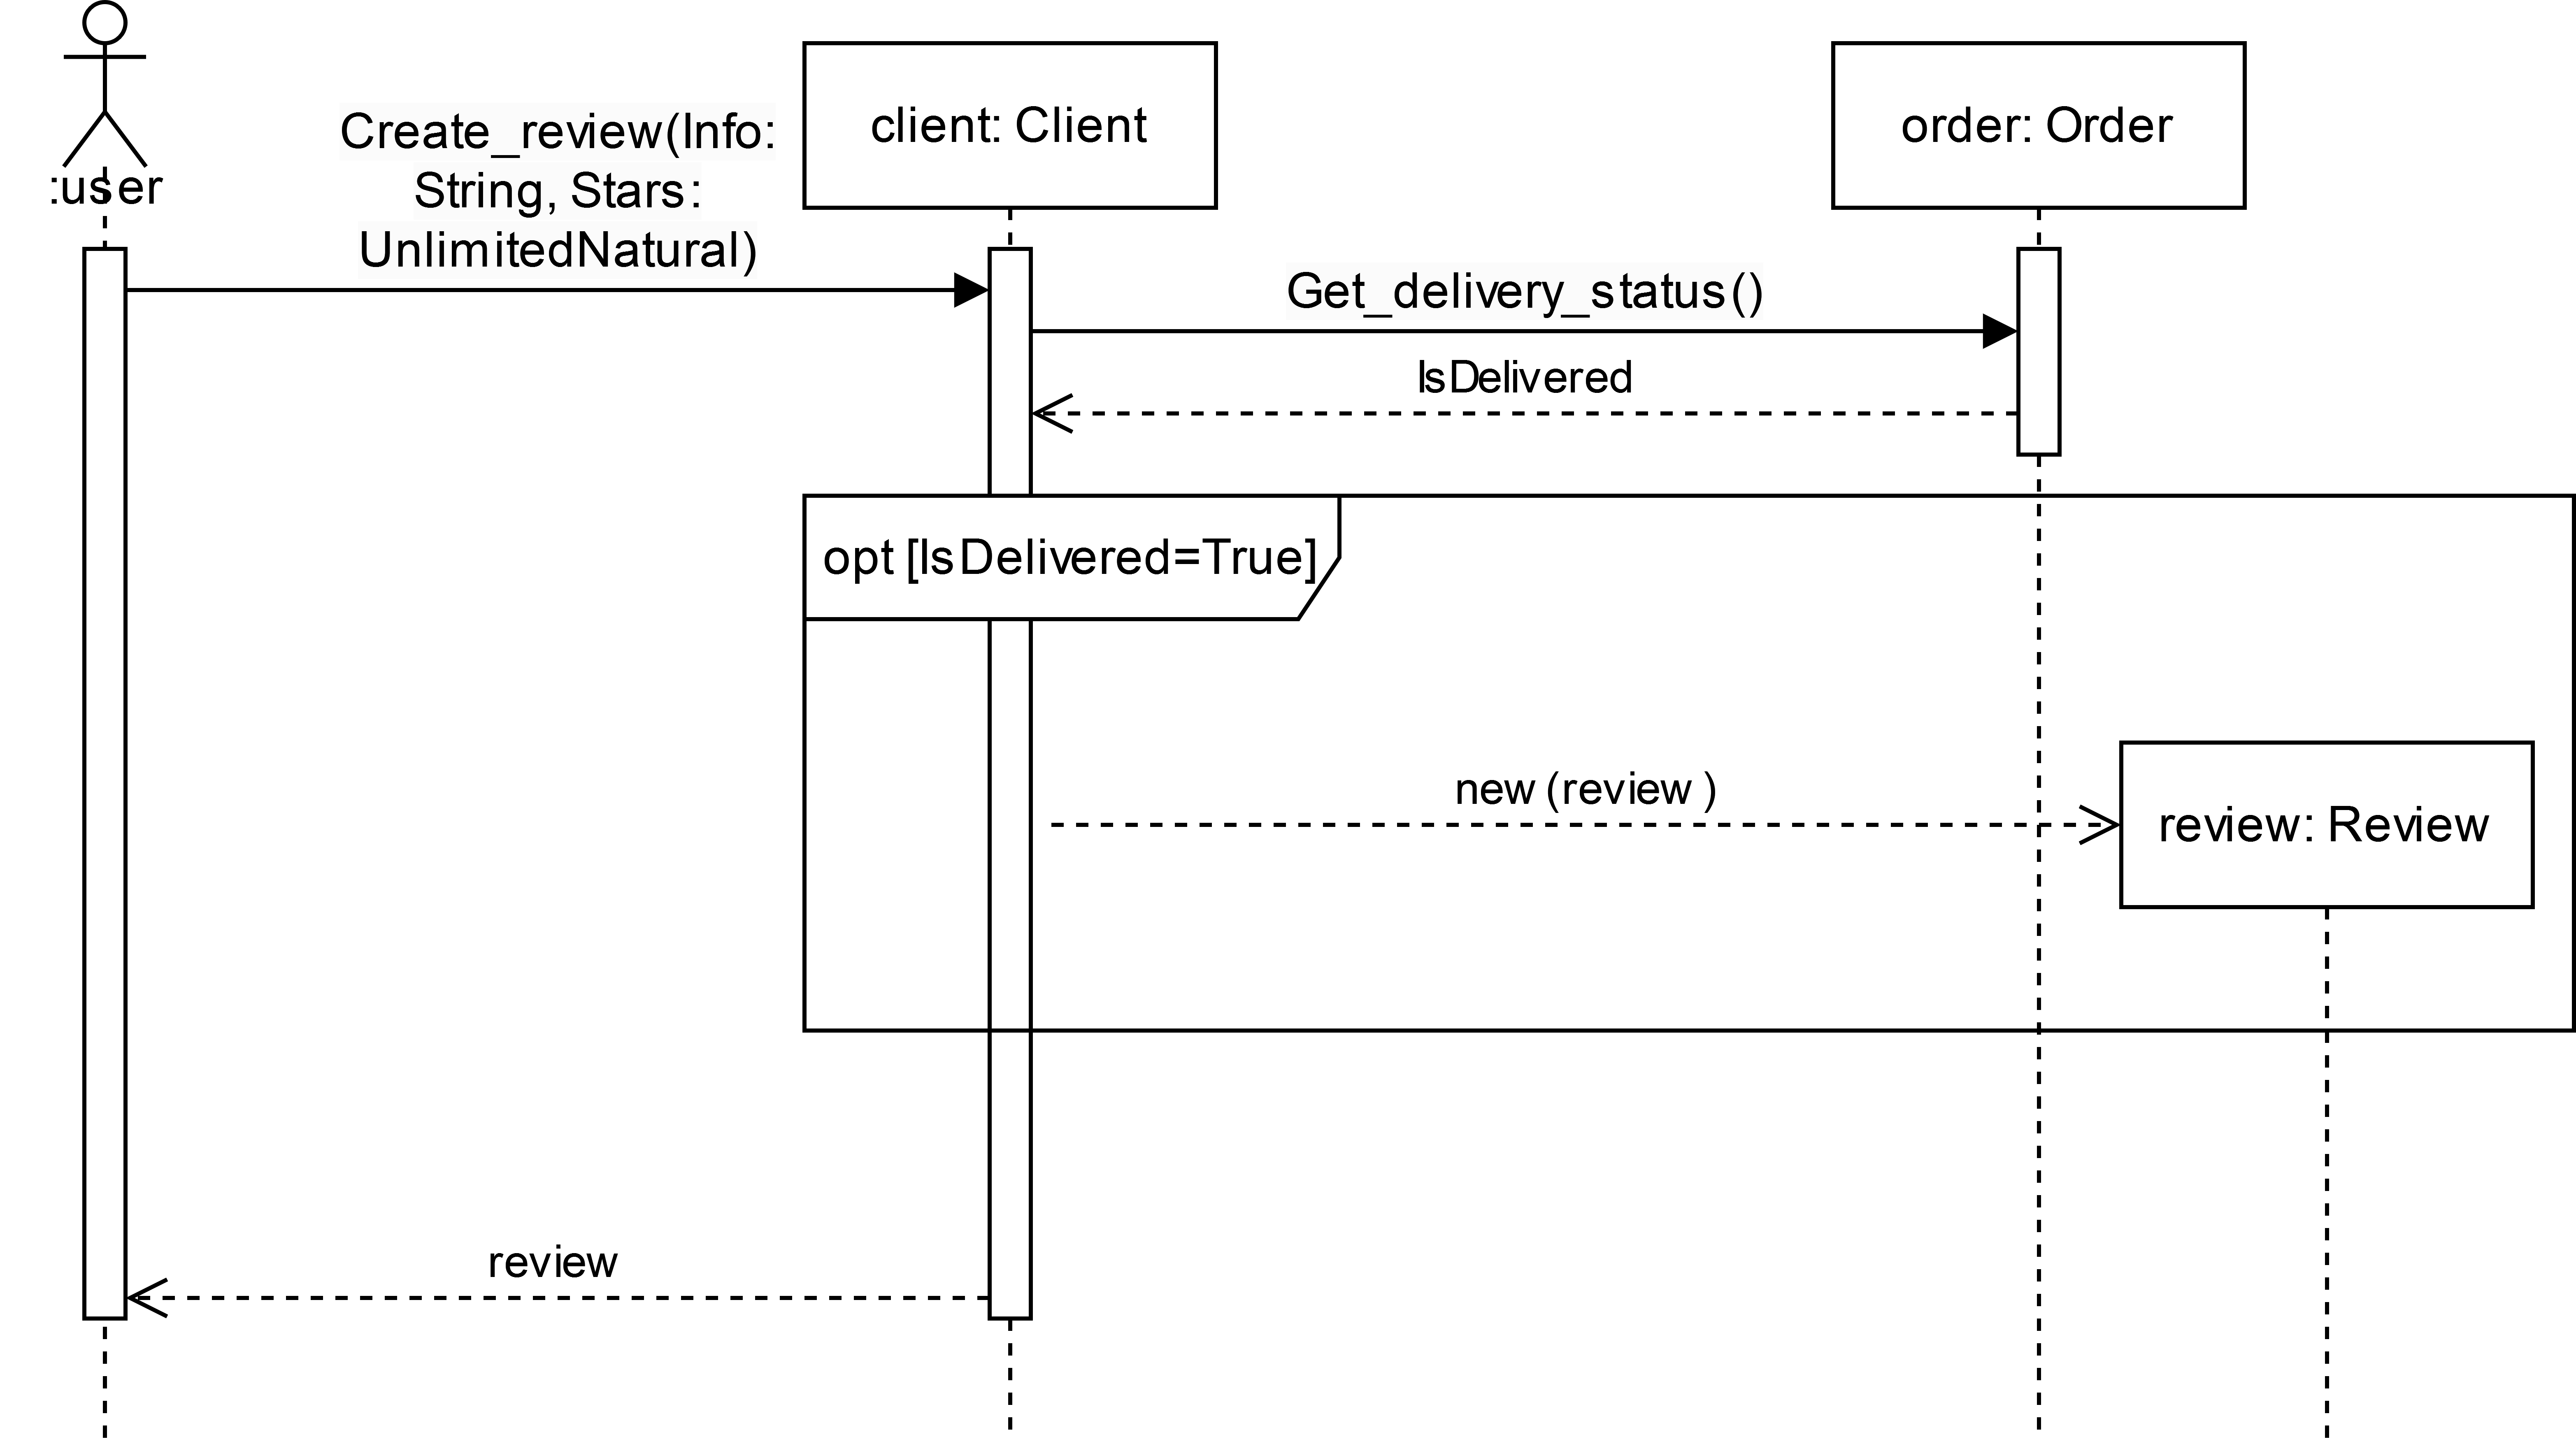
\includegraphics[width=\textwidth]{Диаграмма последовательностей create_review.png}
\end{figure}
User вызывает метод CreateReview у объекта client класса Client. Получается информация о статусе заказа с помощью метода Get\_delivery\_status. Если заказ доставлен IsDelivered = True, то новый объект review типа Review

\subsection{RegisterEmploy}
\begin{figure}[H]
    \centering
    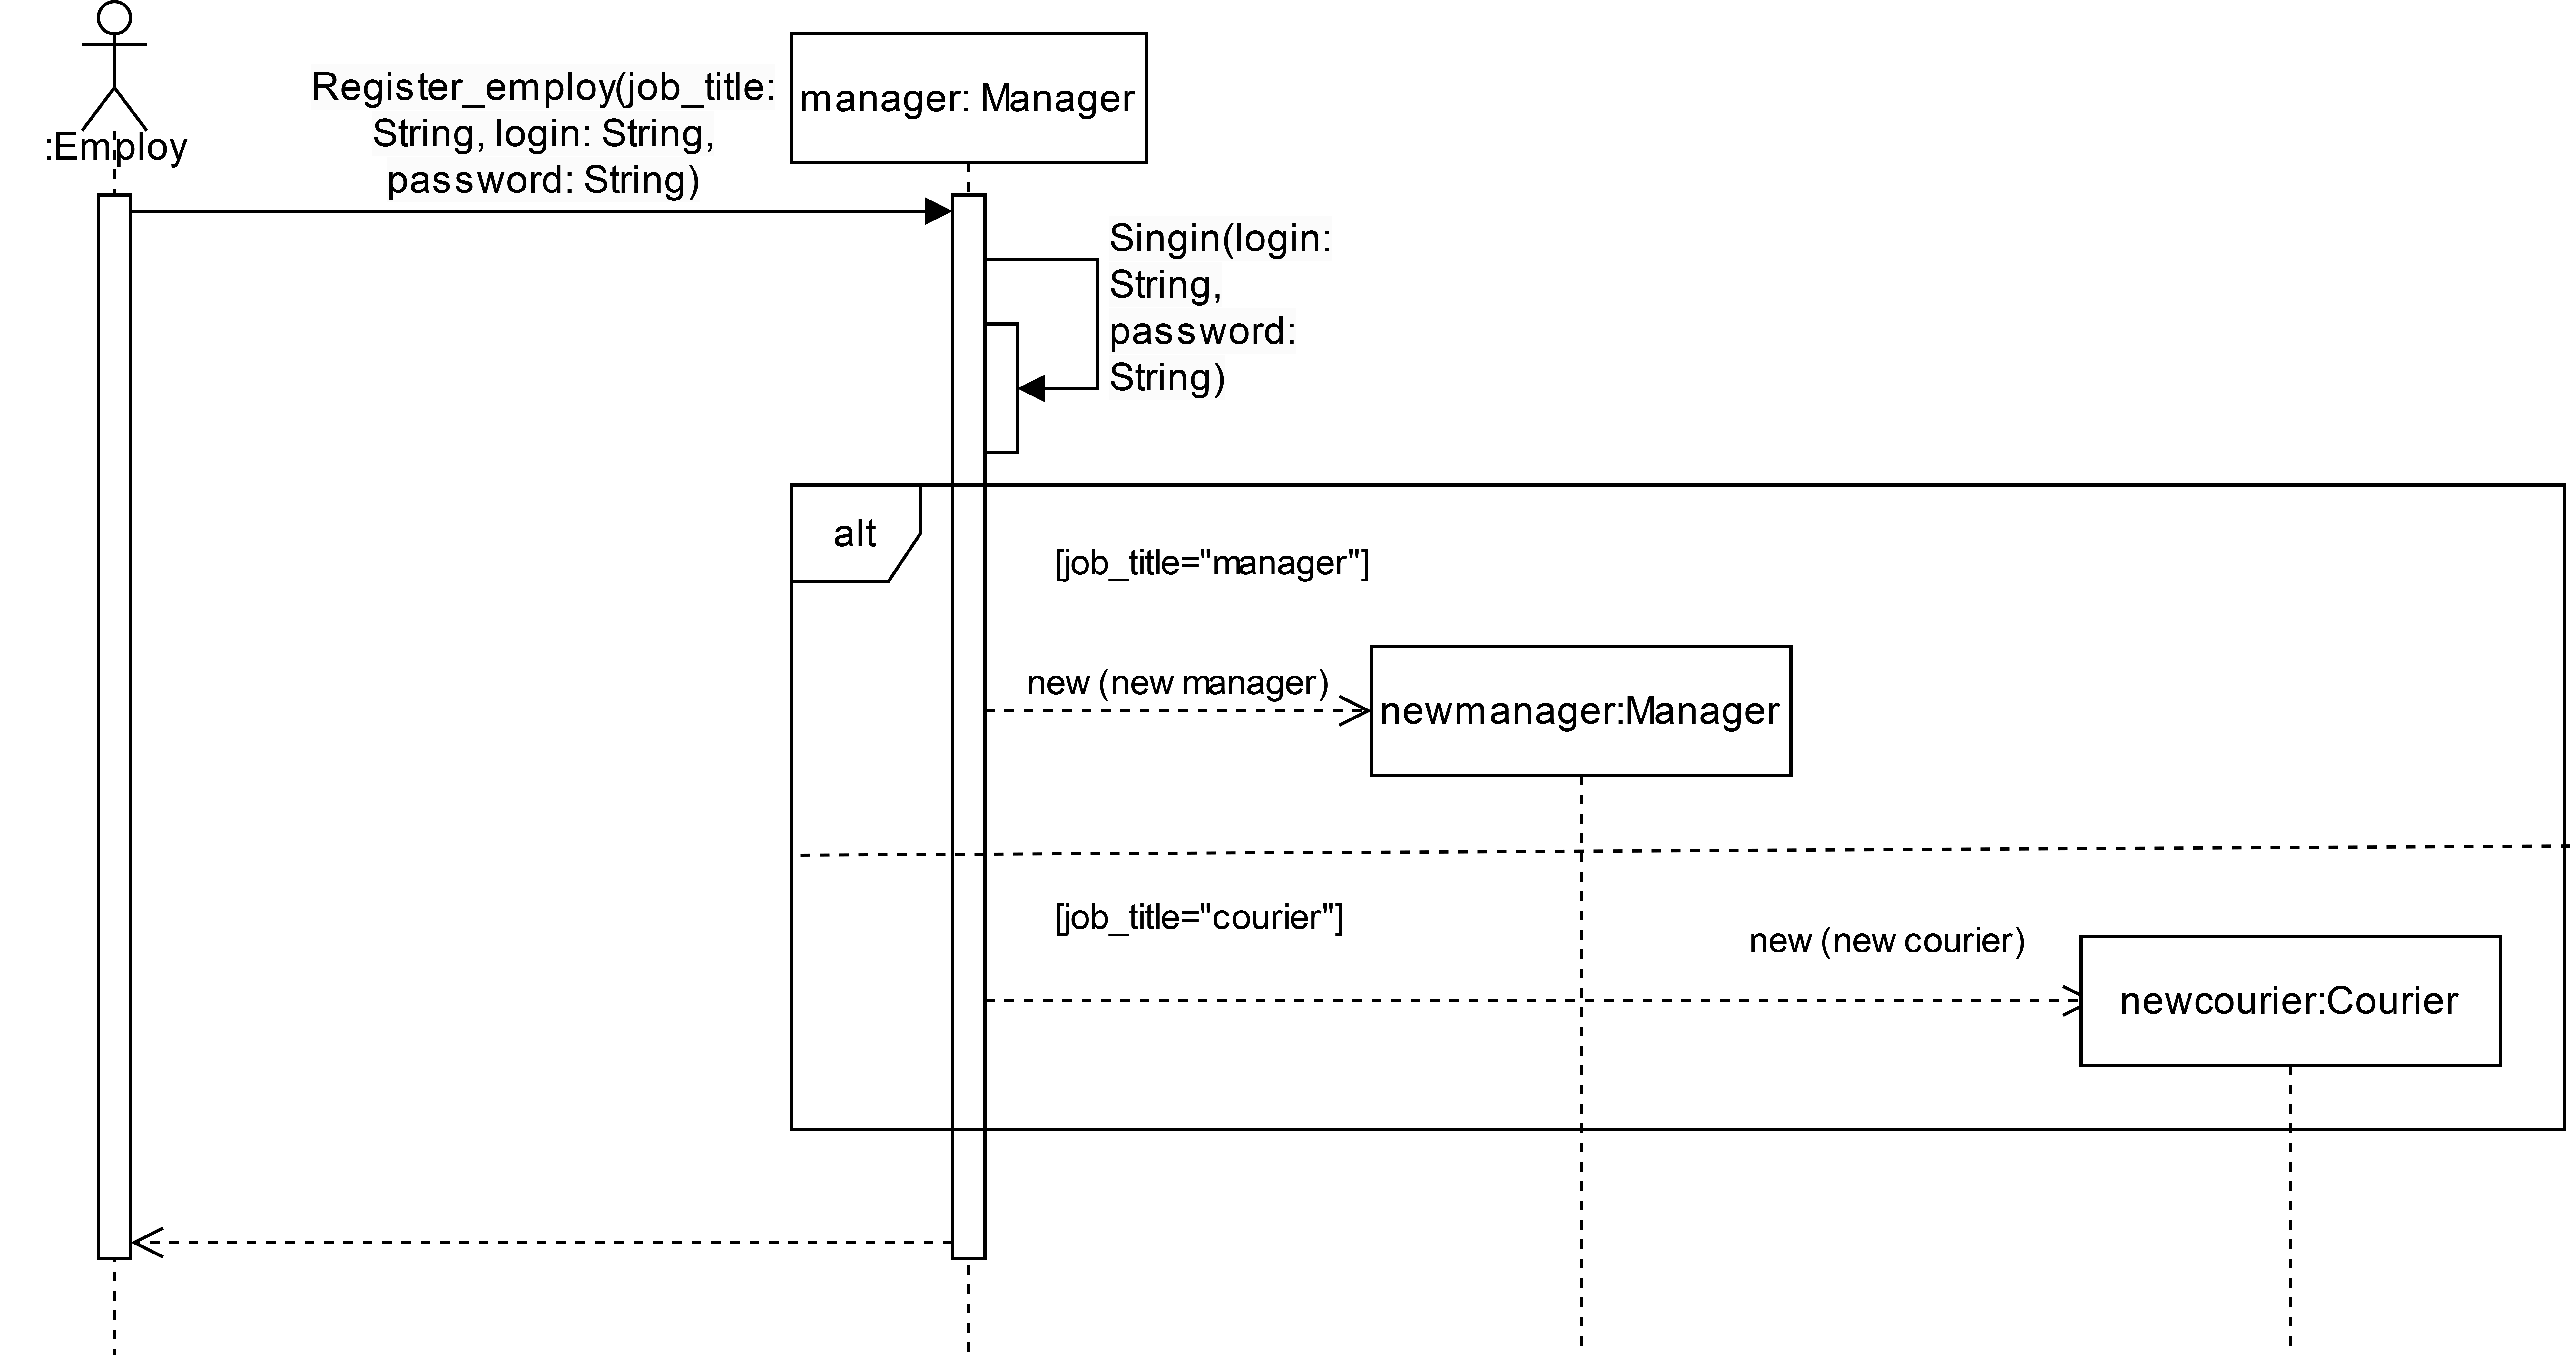
\includegraphics[width=\textwidth]{Диаграмма последовательностей register_employ.png}
\end{figure}
Employ вызывает метод RegisterEmploy у объекта manager класса Manager. Объекта manager начинает новую активность вызывая метод singin у себя. Если job\_title = "manager", то создаётся новый объект newmanager типа Manager, если job\_title = "couirier", то создаётся новый объект newcourier типа Courier

\newpage
\section{Диаграмма объектов}
\begin{figure}[H]
    \centering
    \includegraphics[width=\textwidth]{Диаграмма объектов.png}
\end{figure}
У клиента Petr имеется два заказа Order1 и Order2. Order1 имеет отзыв Review1 и два продукта Котлеты и Куринная грудка. Order2 имеет отзыв Review2 и два продукта Пельмени и Куринные ножки
\newpage
\section{Код}
\inputminted[breaklines]{cs}{main.cs}

\end{document}